\documentclass[letterpaper,12pt]{article}

\title{A Markov Chain Model of Metastasis}
\author{Jack Conger, Minjung Kim, and Mallika Mathur}

\usepackage[margin=2.3cm]{geometry}
\usepackage{amsmath}
\usepackage{amsfonts}
\usepackage{amsthm}
\usepackage{pgfplots}
\usepackage{kbordermatrix}
\pgfplotsset{compat=1.5.1}

\newcommand{\vect}[1]{\boldsymbol{#1}}
\newcommand{\reals}{\mathbb{R}}

\begin{document}

\maketitle

\section{Abstract}

Recently, there has been a growing body of literature in oncology that suggests metastasis is a multidirectional process (where organs metastasize to themselves as well as other organs), overturning a century old belief that it is strictly unidirectional . Much of the literature has suggested there to be clinical evidence of multi-directionality; therefore our Markov Chain model (based on Newton’s) is a viable and valuable approach in modeling what multi-directionality would look like in the human body. This mathematical model can aid surgeons and oncologists in choosing treatments.

\section{Background}

\subsection{Metastasis} %% Minjung

Cancer is a blanket term for numerous different diseases, all characterized by abnormal cell growth. While healthy cells have limitations on their division, as well as pre-programmed death known as apoptosis, cancerous cells spread uncontrollably, interfering with the normal functioning of the rest of the body. Clinically, progression of cancer is classified in four stages, and the fourth stage is usually fatal for the patient. This fatal stage is characterized by metastasis, the spread of cancerous cells from the original tumor to other sites of the body. 

Cancerous cells contained in a single organ are benign and treatable by surgery. A primary tumor within an organ does not have access to the blood vessel (Figure 1), which means that the cells do not have a source of nutrition and stay within the organ and stay weak. When these cells have access to the blood vessel (Figure 2), the cells can grow rapidly, take the nutrition from the non-cancerous cells, prevent them from performing necessary bodily functions, and eventually kill them. With sufficient nutrition, the cancerous cells form blood vessels around themselves in a process called angiogenesis (Figure 3), which gives them more nutrition and allows them to multiply even faster and kill more healthy cells. When metastatic cells are present, it is an indication that the initial tumor has access to the blood vessel and will soon take over the initial organ. Then the metastatic cell can latch onto another organ and multiply to take over another organ. This chain of events will allow the cancerous cells to take over the entire body, shut down all of the organs, and cause death for the patient. 

\begin{figure}
\centering
\begin{minipage}{.3\textwidth}
  \centering
  \includegraphics[width=50mm]{fig1.png}
\caption{A tumor}
\end{minipage}
\begin{minipage}{.3\textwidth}
  \centering
  \includegraphics[width=40mm]{fig2.png}
\caption{Access to blood}
\end{minipage}
\begin{minipage}{.3\textwidth}
  \centering
  \includegraphics[width=35mm]{fig3.png}
  \caption{Angiogenesis}
\end{minipage}
\end{figure}

Due to this nature of metastasis, stopping or delaying metastasis is critical in saving the patients’ lives. The study of cancer metastasis dates back to 1889, when a surgeon named Stephen Paget proposed the ``seed and soil'' model (1). Paget studied over 900 autopsy reports and noticed that the metastasis seemed systematic and non-random. This finding led him to believe that certain initial tumors, which he dubbed “seeds”, were more suited to specific organs’ environments, which he called the ``soil''. These ``seeds'' were more likely to stick onto the organ and start the process of angiogenesis (when the tumor cell starts forming new blood vessels to support the growth of more tumor cells). Although Paget's ``seed and soil'' proposal has been challenged and scrutinized for over a century, it still stands as of today, and it is the proposal that we will use to base our study.

With current research in the field, we now know that there are circulating tumor cells (CTC), the seeds of the Paget model. They are cells from the initial tumor that travels in the bloodstream. CTCs are an example of a biomarker. Making a prognosis is similar to solving a mystery. Just as detectives use fingerprints and footprints to identify a culprit, doctors and surgeons use biomarkers to diagnose a disease. A CTC in the blood stream is an indicator of an initial tumor. Although CTCs are great biomarkers of cancer metastasis, they are a needle in a haystack: a single CTC is hidden in the midst of billion blood cells (2). Currently, there are no efficient ways to detect CTCs in the blood stream. Therefore, there is a clinical need to predict and analyze the movement of CTCs throughout the body.

This metastatic process is a dichotomy: the unidirectional metastasis, where CTCs plant themselves in other organs or there is the multidirectional metastasis, where the CTCs seed other organs or as well as itself (6). Paget's postulate did not include multidirectional metastasis, but the literature suggests that there is a consensus within the scientific community that metastasis is a multidirectional process (6, 7, 8). Although self-seeding may seem insignificant, it has shown to expedite the tumor growth (3) and must be included in the metastatic scenario. Using the seeding model, Newton (4) categorizes organs as either sponges or spreaders. A sponge is an organ that self-seeds and drives the unidirectional metastasis while a spreader is an organ that spreads the CTCs to other organs and contributes to the multidirectional metastasis.

\subsection{Markov Chains} %% Mallika

\subsubsection*{Definitions}

We will use a simple example to illustrate the important definitions:

John is either happy or pouting (a simple soul, our John). If he is happy one day, he is happy the next day four times out of five. If he is pouting one day, the chances that he will also pout the next day are one time out of three. Over the long term, what are the chances that John is happy on any given day?

\begin{enumerate}

\item \textbf{Stochastic process}---A probabilistic (non-deterministic) system that evolves with time via random changes to a collection of variables.

John's happiness is a stochastic process. 

\item \textbf{Finite stochastic process}---A stochastic process with consists of a finite number of stages in which the outcomes and associated probabilities at each stage depend on the outcomes and associated probabilities of the preceding stages.

John's happiness is a finite stochastic process because the outcomes (happy or pouting) and the associated probabilities at each stage depend on the outcomes and associated probabilities of the preceding stages. 

\item \textbf{Markov property}---The probabilities at any stage of a process that satisfies the Markov property depend only on the outcomes of the preceding stage.

John's happiness satisfies the Markov property because his mood depends only on his mood the previous day. 

\item \textbf{Markov chain}---A finite stochastic process that satisfies the Markov property.

John's mood can be modeled by a Markov chain.

\item \textbf{Transition probabilities}---The probabilities associated with the transition from one state to the next in a Markov process:
\begin{align*}
P(\mbox{happy} | \mbox{happy} ) &= 4/5 \\
P(\mbox{pouting} | \mbox{happy}) &= 1/5 \\
P(\mbox{happy} | \mbox{pouting}) &= 2/3 \\
P(\mbox{pouting} | \mbox{pouting}) &= 1/3
\end{align*}

\item \textbf{Transition matrix}---A matrix that summarizes the transition probabilities for a Markov chain. The transition matrix consists of the probabilities of moving from each state to each other state in one time step. If the probability of moving from state $i$ to state $j$ in one time step is $P(\mbox{state }j | \mbox{state }i) = P_{i, j}$ then the transition matrix is
\[
P = \left( \begin{array}{ccccc}
p_{1,1} & p_{1,2} & \cdots & p_{1, j} & \cdots \\
p_{2,1} & p_{2,2} & \cdots & p_{2, j} & \cdots \\
\vdots & \vdots & \ddots & \vdots & \\
p_{i, 1} & p_{i, 2} & \cdots & p_{i, j} & \cdots \\
\vdots & \vdots & & \vdots & \end{array} \right)
\]

The transition matrix for John's mood is
\[
\left( \begin{array}{cc} 4/5 & 1/5 \\
2/3 & 1/3 \end{array} \right)
\]

A transition matrix satisfies the following properties

\begin{enumerate}

\item $0 \leq p_{i, j} \leq 1$ for all $i$ and $j$
\item The sum of the entries in each row is 1
\end{enumerate}

\item \textbf{Distribution vector}---$X_0 = (p_1, p_2, ..., p_n)^T$.

\item \textbf{Finding the probability distribution after $m$ observations}---
If $T$ represents the $n \times n$ transition matrix associated with the Markov process, then the probability distribution after $m$ observations is given by
\[
X_m = T^m X_0.
\]
The probability distribution is described by matrix multiplication because it is found by calculating the conditional probability for each outcome, which is given by the dot product of a row of the transition matrix with the distribution vector (which is a column vector). 

\item \textbf{Steady-state distribution vector}---As the number of observations increases, the probability distribution vector approaches a vector called the steady-state distribution vector. 

\item \textbf{Steady-state Matrix}---The powers $T^m$ of the transition matrix $T$ tend toward a fixed matrix $L$ as $m$ increases. $L$ is called the steady-state matrix. 

The steady state is reached regardless of the initial state of the system.

\end{enumerate}

\subsection{Singular Value Decomposition (SVD)}

Singular value decomposition is a method used to diagonalize an $n \times m$ matrix $A$---where, thus, $A$ is a transformation mapping $\reals^n \to \reals^m$. We can easily find an orthonormal basis for $\reals^n, V = (\vect{v}_1, \vect{v}_2, ..., \vect{v}_n)$, by using Gram-Schmidt orthogonalization, and see how this basis is morphed for the codomain $\reals^m$ into $U = (\vect{u}_1, \vect{u}_2, ..., \vect{u}_m)$. This looks like
\[
A(\alpha_1 \vect{v}_1 + \alpha_2 \vect{v}_2 + ...) = \sigma(\beta_1 \vect{u}_1 + \beta_2 \vect{u}_2 + ...)
\]
\[
AV = U\Sigma,
\]
where $\Sigma$ is the diagonal matrix with entries $\Sigma_{i,i} = \sigma_i = \sqrt{\lambda_i}$ with $\lambda$ the eigenvalues of $A^T A$, indexed from largest to smallest. We then know that
\[
A = U \Sigma V^{-1},
\]
but since the vectors in $V$ are all orthonormal,
\[
A = U \Sigma V^T.
\]

Geometrically, the singular values indicate the distortion of data given by $L_A$. For instance, for certain special cases of the matrix $A$, $U$ and $V^T$ represent rigid rotations, while $\Sigma$ is a stretching matrix; then, we can characterize $A$ as the composition of a rotation, stretch, and rotation. Then, in this case, the singular values are the various ways of ``stretching'' which occurs to the vector being transformed. In general, this characterization is not true, but it provides a good illustrative example for what role singular values perform.

Therefore in our case, calculating the standard deviations of singular values of our set of 1000 transition matrices (see Methodology) will allow us to assess the validity of the set, in that smaller standard deviations would indicate that the matrices distort the data similarly and show that there is a general unidirectional path of the cancer cells.

\section{Why use Markov Chains?}

Markov chain methodology is a very convenient and powerful modeling tool for those stochastic processes which satisfy the Markov property; given that something \emph{does} satisfy this property, Markov chains should likely be a first candidate for modelling. Fortunately, cancer metastasis does seem to satisfy the conditions required for using Markov chains.

Firstly, CTCs are relatively rare compared to healthy cells and, moreover, difficult to track. Currently in the field, there is a consensus that CTCs are stochastic---we can only predict, probabilistically, where the seeds and soils may be.

Further, metastasis can be considered a \emph{finite} stochastic process; each stage in a hypothetical Markov chain model represents a metastatic stage as the cancer spreads, as the CTCs find ``soil'' in each new location throughout the body.

The last, and most crucial, condition for using Markov chains is the Markov property. It is thought that the the behavior of CTCs is relatively homogeneous, depending only on their location and hypothetically the type of tumor; this means that the current state of the system---that is, where the tumors currently exist---is the primary, if not only, determining factor of the evolution of the system. Thus, we can use a Markov chain as a model.

There are a few implications and complications of using Markov chains for our model:

\begin{itemize}

\item It is important to note that because we have no frame of reference for the speed of metastasis, our model is not connected to real time. While John's moods change once a day, each stage of the metastasis ravaging his body may be months apart or minutes apart, depending on the unpredictable nature of seeding of CTCs. Newton et al \cite{newton}

This means that our model cannot imply real-time consequences without other, additional information. However, we can refer, in-model, to how cancer spreads \emph{relatively} within different parts of the body.

\item Because of the nature of our \emph{a priori} data, our process will be slightly backwards. A typical problem involving a Markov chain is stated as follows:

\emph{Starting from one state of a process (the current state), determine the probability that the process will be at a particular state at some future time.} 

In this type of problem, the transition matrix is given, and the goal is to find the steady-state vector. However, our goal is the converse of the above typical problem. We are given the metastases of the body at its final, long-term point (death), and from this long-term state, we want to discern the transition matrix. The details of our process are given in section 5.1; however, the somewhat-backwards nature of our goal should be stated clearly.

\item We can model the time it takes for cancer from a primary tumor to metastasize to a certain organ using a tool called \emph{mean first-passage times}, or mfpt:

Given a starting index and a transition matrix, we perform a ``random walk'', assigning new locations stepwise according to our probability distributions, until we reach our target index. The number of steps taken to reach this is the ``first-passage time'', which can be calculated repeatedly and averaged.

In our model, these mfpts represent how long it takes cancer to metastasize from a certain primary tumor to a site in question. This, in turn, has implications for diagnosing and treating cancer in a patient's body: those organs with lower mfpts would be tested first.

\end{itemize}

\section{Goal}

Our goal is to replicate Newton's results and identify which organs are sponges and spreaders for lung cancer metastasis. To do this, we will use the data they use to calculate a transition matrix, from which we will find the sponges and spreaders. We will also calculate mean first passage times of the organs.

\section{Methodology}

To study the natural movement of metastatic cells throughout the body, we used the raw data from an autopsy report of untreated cancer patients from the early 1900s (9). Metastases from 32 initial tumor sites were verified by examination and histology and added up in a form of a matrix $M_{i,j}$ where organs in $i$ were the organs of the initial tumor and the organs in $j$ were the organs of the metastases.

\subsection{Finding the Transition Matrix}

The steady-state, or long-time, distribution vector of a Markov Chain is given by 
\begin{align}
\lim_{k \to \infty} \vect{v}_0 A^k = \vect{v}_\infty,
\end{align}
and is thus characterized by the fact that
\begin{align}
\vect{v}_\infty A = \vect{v}_\infty
\end{align}
We assume this steady-state distribution to be the same as the distribution of metastases obtained from the data, $\vect{v}_T$ (the ``target'' vector). However, the data provides no transition matrix which will result in this distribution. And (following Newton's methodology) because we lack enough information to analytically create a transition matrix, we will start with a $50 \times 50$ ``best guess'' matrix $A_0$ and modify it until we obtain a matrix which will converge to the steady-state.

$A_0$, the initial best-guess matrix, will be constructed as follows: each column and row corresponds to an organ of interest in the autopsy data. For the row corresponding to the cancer we are interested in (in Newton's paper, lung cancer,) we will use the metastasis distribution for that type of cancer. For the other rows, we will use the general metastasis distribution over all cancers in the autopsy.

Newton's paper, and a quick check, show that this matrix will not lead to convergence to $\vect{v}_T$. However, we know that if given the right $A$, then by (2) above,
\begin{align*}
\vect{v}_T A &= \vect{v}_T \\
\vect{v}_T A - \vect{v}_T &= \vect{0} \\
\vect{v}_T (A - I) &= \vect{0}.
\end{align*}
Knowing this, we can find $A$ by minimizing whatever residual value $\vect{r}$ falls on the right side of the equation. To duplicate Newton's results, we will set a threshold at $\epsilon = 10^{-5}$, where, if $\| \vect{r} \|^2 \leq \epsilon$, we will be satisfied with our $A$.

Before we determine this matrix, it should be stated that we have two constraints on $A$:
\begin{itemize}
\item $0 \leq a_{ij} \leq 1$, since each value in $A$ is a probability, and
\item $\sum_{j = 1}^{50} a_{ij} = 1$, by the nature of Markov chains.
\end{itemize}
With this in mind, we calculate the matrix $A$ iteratively using the following algorithm, starting with our $A_0$:
\begin{enumerate}
\item For our $A_j$, calculate $\vect{r}_j$.
\item Find the column $k$ of $A_j$ corresponding to the maximum entry of $\vect{r}_j$.
\item Find the column $l$ of $A_j$ corresponding to the minimum entry of $\vect{r}_j$.
\item Choose a random row $i$ of $A$.
\item Obtain $A_{j + 1}$ by decreasing the maximum entry $(a_{ik})$ by $\delta$, and increase the minimum entry $(a_{il})$ by $\delta$, where $\delta$ is set as $d \| \vect{r}_j \|^2$, with $d$ an arbitrary scaling constant.
\item Calculate $\vect{r}_{j+1}$.
\item Repeat steps 2-6 as long as $\| \vect{r}_{j + 1} \|^2 > \epsilon$.
\end{enumerate}

We repeat this one thousand times to obtain an ensemble of transitional matrices, and then average these to make a single ensemble matrix. Additionally, we calculate each matrix's singular values and create distributions for each one: this will allow us to determine the similarity or difference in data distortion caused by the matrices (see 2.3).

\subsection{Identifying the Sponges and Spreaders}

This is a simplified transition matrix with just three organs. We will use this matrix to illustrate our method for identifying sponges and spreaders. (The probabilities in this matrix are arbitrary, not the actual data.)

\[
  T=\kbordermatrix{%
      & lung &  liver & bone \\
    lung & .1 & .4 & .5 \\
    liver & .5  & .2 & .3 \\
    bone & .7 & .1 & .2
  } 
\]

Each element in $T$, $t_{i,j}$, represents the probability that the cancer will metastasize from organ $i$ to organ $j$. For example, the probability that the cancer will metastasize from the
bone to the lung is .7. 

To identify whether an organ is a sponge or a spreader, we will calculate two probabilities, $P_{out}$ and $P_{in}$. 

$P_{in}$ is the probability of metastatic cells entering a single organ, which we will denote as organ $j$. In this $3 \times 3$ example, 
$P_{in} = (\sum_{i=1}^{3}t_{i, j}) - t_{j, j}$

$P_{out}$ is the probability of metastatic cells traveling to other organs from a single organ that we will denote as organ $i$. In this $3 \times 3$ example,

$ P_{out} = (\sum_{j=1}^{3}t_{i, j}) - t_{i, i}$

Then, we will calculate the ratio $P_{out}/P_{in}$. If this ratio is greater than 1, it is called an amplification factor 
and it indicates that the organ is a spreader. If it is less than 1, it is called the absorption ratio and it indicates that the organ is a sponge. 

In this particular example,
\[
P_{out} = .5 + .3
\]
\[
P_{in} = .4 + .1
\]
\[
\mbox{Ratio} = .8 / .5 = 1.6
\]

The ratio is greater than 1, so it is called an amplification factor. So, this transition matrix would indicate that the liver is a spreader. 

\subsection{Mean First Passage Time (mfpt)}

Determining the mean first-passage time to each location is an example of using a ``random walk'' algorithm. Using our transition matrix and starting at a certain point, we perform the following steps in order to determine the mfpt for a certain organ:

\begin{enumerate}
\item Determine the probability distribution $\vect{p} = (p_1, p_2, ..., p_n)$ of our current location (the corresponding row of the transition matrix)

\item Calculate $\vect{p}' = (p_1', p_2', ..., p_n')$, the cumulative distribution vector, such that
\begin{align*}
p_1' &= p_1 \\
p_2' &= p_1 + p_2 \\
p_3' &= p_1 + p_2 + p_3 \\
\vdots \\
p_n' &= p_1 + p_2 + ... + p_n
\end{align*}

\item Find a random number $x$ between 0 and the sum of the elements in $\vect{p}$ (this should be 1, but due to floating point errors, may be slightly different, and so should be accounted for in the calculation).

\item Iterate over the elements of $\vect{p}'$: the index $k$ of the first value for which $p_k' \geq x$ is the new location.

\item Repeat until the reached location is the same as the target. The number of iterations required to reach this point is the first-passage time.

\end{enumerate}

This is calculated a large number of times and the times are averaged to find the mfpt for that organ. This calculation is performed for each location, to determine which organs tend to be metastasized to first, and which tend to be later.

\section{Results}

We determined an ensemble transition matrix, and the singular values of them, plotted in Fig. 4. The graph of the mean 27 singular values and their standard deviations show that the set of 1000 matrices are similar. As expected, the singular values are in a decreasing order, and the small standard deviations show that the set of matrices generally distort the data similarly. These two observations are reassuring signs that the set is sufficiently homogenized.

There were a few decisions to be made regarding the transition matrix. For one thing, we chose our scaling factor $d$ (in step 5 in section 5.1) to be 100. This had the effect of increasing the standard deviation of our singular values---and, indeed, they are somewhat more varied than those in Newton's study. However, it created a more strongly-mixing transition matrix, which we decided to be somewhat more important than an extremely low variance.

Additionally, our transition matrix ($50 \times 50$) had twenty columns with elements all zero. These locations, because they could not be metastasized to from the lungs, thus had their columns and rows removed, leaving us with a $30 \times 30$ matrix.

\begin{figure}[h!]
	\centering
	\begin{tikzpicture}
		\begin{semilogyaxis}[width=\textwidth, xlabel=Index,ylabel=Singular Values,ymin=0,ymax=2.5,xmin=-1,xmax=28]
		\addplot[mark=x, draw=none, error bars/.cd, y dir=both, y explicit] coordinates { % averages
			(0, 2.109) +- (0.0454, 0.0454)
			(1, 0.548) +- (0.1099, 0.1099)
			(2, 0.389) +- (0.0625, 0.0625)
			(3,0.302) +- (0.05143, 0.05143)
			(4,0.238) +- (0.04417, 0.04417)
			(5,0.194) +- (0.03407, 0.03407)
			(6,0.163) +- (0.02646, 0.02646)
			(7,0.139) +- (0.02083, 0.02083)
			(8,0.119) +- (0.01812, 0.01812)
			(9,0.1020) +- (0.01565, 0.01565)
			(10,0.0871) +- (0.01321, 0.01321)
			(11,0.0740) +- (0.01079, 0.01079)
			(12,0.0628) +- (0.00889, 0.00889)
			(13,0.0530) +- (0.00809, 0.00809)
			(14,0.04416) +- (0.00677, 0.00677)
			(15,0.03646) +- (0.00569, 0.00569)
			(16,0.030528) +- (0.00424, 0.00424)
			(17,0.02598) +- (0.00304, 0.00304)
			(18,0.022521) +- (0.00245, 0.00245)
			(19,0.019627) +- (0.00202, 0.00202)
			(20,0.0171385) +- (0.00180, 0.00180)
			(21,0.0147789) +- (0.00171, 0.00171)
			(22,0.012491) +- (0.00162, 0.00162)
			(23,0.010382) +- (0.00153, 0.00153)
			(24,0.00841735) +- (0.00130, 0.00130)
			(25,0.00680907) +- (0.00108, 0.00108)
			(26,0.00541237) +- (0.00094, 0.00094)
			(27,0.00400775) +- (0.00083, 0.00083)
		};
		\addplot[mark=-, draw=none] coordinates { % lower bound s.d.
			(0, 1.9377)
			(1, 0.3031434)
			(2, 0.210476)
			(3,0.1717717)
			(4,0.135643806)
			(5,0.117742)
			(6,0.10007)
			(7,0.087246)
			(8,0.06207)
			(9,0.053537)
			(10,0.0495463)
			(11,0.045576)
			(12,0.035099)
			(13,0.032145)
			(14,0.02679)
			(15,0.023770)
			(16,0.02027212)
			(17,0.018855)
			(18,0.01548364)
			(19,0.013498)
			(20,0.01180723)
			(21,0.0094616)
			(22,0.006911)
			(23,0.00588717)
			(24,0.00472875)
			(25,0.00396749)
			(26,0.002676405)
			(27,0.0016137)
		};
		\addplot[mark=-, draw=none] coordinates { % upper bound s.d.
			(0, 2.3119)
			(1, 0.9766)
			(2, 0.61454)
			(3,0.500328)
			(4,0.3892882)
			(5,0.31233635)
			(6,0.2774090)
			(7,0.249448)
			(8,0.20795)
			(9,0.18389)
			(10,0.1316879)
			(11,0.1213676)
			(12,0.094492)
			(13,0.0815786)
			(14,0.0671606)
			(15,0.05814518)
			(16,0.047392)
			(17,0.040841)
			(18,0.0304549)
			(19,0.025638)
			(20,0.0234585)
			(21,0.0207625)
			(22,0.017494)
			(23,0.015214875)
			(24,0.0128207492)
			(25,0.01050695)
			(26,0.0082212242)
			(27,0.0072167757)
		};
		\end{semilogyaxis}
	\end{tikzpicture}

	\caption{Plots of the first 27 singular values, from largest to smallest, of the ensemble transition matrix. The $\times$ marks are mean values, the error bars are standard deviation, and the disconnected dashes are minimum-maximums.}
\end{figure}

Using this transition matrix, we then calculated the spreaders and sponges from primary lung cancer:

\textbf{Spreaders}---Bladder, brain, breast, diaphragm, gall-bladder, heart, large intestine, omentum, ovary, pericardium, peritoneum, prostate, skeletal muscle, skin, small intestine, spleen, stomach, testes, thyroid, uterus, and vagina.

\textbf{Sponges}---Adrenal, bone, kidney, liver, lung, lymph nodes (both distant and regional), pancreas, and pleura.

However, some of the results we obtained seemed abnormally high: while Newton noted on high ratios of, say, two, we obtained ratios of over sixty. Something in our implementation seems to have been incorrect.

For our calculations of mfpt, plotted in fig. 5, we were very close to Newton's results. We chose an ensemble size of 200 for a convenient mix of consistency and speed. The thirteen lowest passage times in Newton's paper were regional and distant lymph nodes respectively, adrenal gland, liver, lung, bone, kidney, pleura, pancraes, spleen, heart, and thyroid. Our results were identical, aside from switching the liver and adrenal gland, likely just random difference, and the lack of lung---our algorithm returned a mfpt of zero for lung, because it was the primary cancer. Despite these minor differences, the mfpts were very similar.

\begin{figure}[h!]
\centering
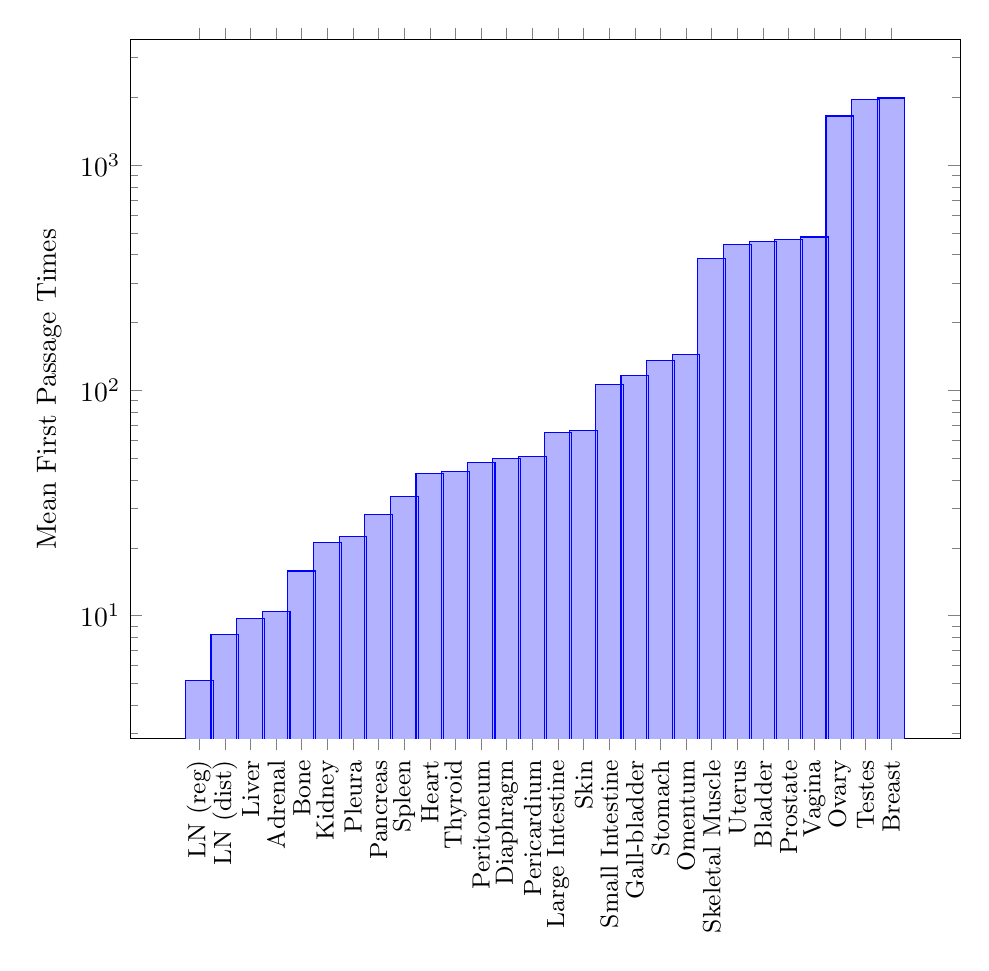
\begin{tikzpicture}
\begin{semilogyaxis}[
width=\textwidth,
symbolic x coords={
LN (reg),LN (dist),Liver,Adrenal,Bone,Kidney,Pleura,Pancreas,Spleen,Heart,Thyroid,Peritoneum,Diaphragm,Pericardium,Large Intestine,Skin,Small Intestine,Gall-bladder,Stomach,Omentum,Skeletal Muscle,Uterus,Bladder,Prostate,Vagina,Ovary,Testes,Breast},
x tick label style={rotate=90, font=\small}, ybar,
xtick=data, ylabel={Mean First Passage Times}
]
		\addplot coordinates {
			(LN (reg),5.155)
			(LN (dist),8.235)
			(Liver,9.68)
			(Adrenal,10.39)
			(Bone,15.775)
			(Kidney,21.205)
			(Pleura,22.37)
			(Pancreas,28.14)
			(Spleen,33.68)
			(Heart,42.65)
			(Thyroid,43.79)
			(Peritoneum,47.715)
			(Diaphragm,50.025)
			(Pericardium,50.985)
			(Large Intestine,65.145)
			(Skin,66.525)
			(Small Intestine,105.7)
			(Gall-bladder,116.13)
			(Stomach,135.35)
			(Omentum,143.815)
			(Skeletal Muscle,385.18)
			(Uterus,442.215)
			(Bladder,455.745)
			(Prostate,465.44)
			(Vagina,479.41)
			(Ovary,1651.435)
			(Testes,1951.255)
			(Breast,1985.385)
		};
\end{semilogyaxis}
\end{tikzpicture}

\caption{mfpts of each metastasis site. Note the logarithmic plot.}
\end{figure}

\section{Discussion}

Clinically, the classification of organs into seeders or sponges will allow surgeons to slow down metastasis more effectively. Sponges, self-seeders, have shown to speed up the metastatic process (3). Spreaders, which give rise to metastatic cells, risk the proliferation of cancerous cells. Therefore, metastases in those organs should be surgically removed. For example, Newton et al found that the adrenal gland and the kidney are the spreaders and the lymph nodes, liver, and bone are sponges for lung cancer. More than a decade ago, Bretcha-Boix et al found that surgical removal of adrenal gland metastasis was a successful treatment for patients with lung cancer adrenal metastasis (5). Even without knowing that the adrenal gland was a spreader for lung cancer, Bretcha-Boix et al noticed that the removal of the adrenal metastasis stopped the progression of lung cancer. Although this is just one specific case, it would be valuable for researchers and surgeons to do clinical trials on the effectiveness of treating patients by surgically removing sponges and spreaders to test our hypothesis to see if it prolongs the survival rate.

Another clinical application to consider is the mean first passage time (mfpt). Calculated mfpt tells us the time it takes for the metastatic cell to reach the organ. Newton et al compared the changes in the mfpt between untreated, stage I resection (removing a part of the organ with initial tumor), and stage II resection patients. They found that the untreated and the stage II resection had the negligible differences in mfpt. Meanwhile, the mfpt for stage I resection was sufficiently longer, which means that the resection delayed the progression of the tumor. A feasible way to assess the effectiveness of the treatment without looking at the survival rate (clinically, it could potentially take decades) is to calculate changes in mfpt with resection in various organs. An increase in the slope of the mfpt linear fit increases would indicate prolonged metastasis. If not, that implies that the resection did not have impact on progression and the surgery was unnecessary. To look at specific changes in the pathway of the metastasis, we could also focus on how each organ’s mfpt changes with various treatments.

\section{Implementation}

The following code is written in Python 3.3.1, using the numpy module from www.numpy.org.

This first file calculates the transition matrix.

\begin{verbatim}
import numpy as np
import random
from datetime import datetime as dt

np.set_printoptions(8, 5000, 3, 1000, True, "NaN", "inf", None)

'''
=======================================================
                 VARIABLE DEFINITIONS
=======================================================
'''

# The original FULL dataset for all cancers
orig_data_total = # omitted for conciseness

# the number of tumors of each type of metastasis
type_metas_rate = sum(orig_data_total)
# the total number of metastases
num_metas_total = sum(type_metas_rate)
# the general metastasis distribution (normed)
total_distribution = [l / num_metas_total for l in type_metas_rate]

# the row of the particular primary tumor we care about
primary = 22
# the metastases for the primary cancer we want
orig_data = orig_data_total[primary]

# the normed data for the cancer we want
num_metas = sum(orig_data)
norm_data = [l / num_metas for l in orig_data]

# just the identity matrix
ident = np.eye(len(norm_data))

# calculation constants:
epsilon = 10**(-5) # error size
delta_scale = 100.0 # delta 'scaling'
ensemble_size = 1000 # number of matrices to average



'''
=======================================================
                  FUNCTION DEFINITIONS
=======================================================
'''
# Builds A_0 and begins iteration

def create_matrix():
    mat = np.zeros([len(norm_data),len(norm_data)]) # creates an empty matrix
    for i in range(len(norm_data)): # fills the rows ...
        if i == primary:
            mat[i] = norm_data # ... with the primary distribution
        else:
            mat[i] = total_distribution # ... with the general distribution
        
    mat = iterate(mat) # start iteration
    return mat

# Iterates to get A_f from A_0
def iterate(mat):
    resid = np.dot(norm_data, mat - ident) # calculate residual
    normsq_resid = np.dot(resid, resid)
    
    while normsq_resid > epsilon:
        max_col = np.argmax(resid) # pick max column
        min_col = np.argmin(resid) # pick min column
        row = random.randrange(0, len(norm_data)) # pick row
        delta = normsq_resid * delta_scale # pick delta
        
        if (mat[row][max_col] - delta) < 0: # to prevent values < 0 in matrix
            delta = mat[row][max_col]       

        mat[row][max_col] = mat[row][max_col] - delta
        mat[row][min_col] = mat[row][min_col] + delta

        resid = np.dot(norm_data, mat - ident) # calculate new residual
        normsq_resid = np.dot(resid, resid)

    return mat






'''
=======================================================
                      RUNTIME STUFF
=======================================================
'''

fo = open("results.txt","w+")

# Prints some parameters of calculation
print("Epsilon: " + repr(epsilon))
print("Ensemble size: " + repr(ensemble_size))
print("Delta scale: " + repr(delta_scale))

fo.write("Target distribution: " + repr(norm_data) + "\n")
fo.write("General distribution: " + repr(total_distribution) + "\n")
fo.write("Epsilon: " + repr(epsilon) + "\n")
fo.write("Ensemble size: " + repr(ensemble_size) + "\n")
fo.write("Delta scale: " + repr(delta_scale) + "\n\n")

time1 = dt.now()

print("Calculating matrices ...")

# Creates the first matrix
mat = create_matrix()
mat_list = [mat]

# Creates the rest of the matrices
for i in range(2, ensemble_size + 1):
    nmat = create_matrix()
    mat = mat + nmat
    mat_list.append(nmat)
    if i % 5 == 0:
       print(i, end=" ")

print()

# Calculates the average matrix
print("Averaging ...")
mat = mat / ensemble_size

time2 = dt.now()
dtime = time2 - time1

# Prints the results of the A_j ensemble, and runtime info
difstr = repr(np.dot(norm_data, mat) - norm_data)
difstr = difstr[6:len(difstr)-1]
fo.write(repr(mat) + "\n\n")

fo.write("Difference: " + difstr + "\n")
fo.write("Time: " + repr(dtime.seconds) + "." + repr(dtime.microseconds) + " s\n\n")

fo.write(" ----------------- \n\n")

print("Performing SVD ...")

sval_list = []

for i in range(len(mat)):
    sval_list.append([])

# Calculates the singular values for each matrix
for mat in mat_list:
    sval = np.linalg.svd(mat, False, False)
    for i in range(len(sval)):
        sval_list[i].append(sval[i])

# Prints data about the singular values
for i in range(len(sval_list)):
    fo.write("For value " + repr(i) + "\n")
    fo.write("    Mean = " + repr(sum(sval_list[i]) / len(sval_list[i])) + "\n")
    fo.write("    Median = " + repr(np.median(sval_list[i])) + "\n")
    fo.write("    Min-max = " + repr(min(sval_list[i])) + " -> "
          + repr(max(sval_list[i])) + "\n")
    fo.write("    STDev = " + repr(np.std(sval_list[i])) + "\n\n")

fo.close()

print("Done")

\end{verbatim}

\pagebreak

This second file calculates the sponges and spreaders.

\begin{verbatim}
import numpy as np

names = # labels of organs, too long for inclusion

transition = # the 30x30 transition matrix; again, omitted for conciseness

mat = np.dot(transition,transition)

spreaders = []
sponges = []

for i in range(30):
    p_out = 0

    for j in range(30):
        if i != j:
            p_out = p_out + mat[i,j]

    p_in = 0
    for k in range(30):
        if k != i:
            p_in = p_in + mat[k,i]

    ratio = p_out/p_in
    print(names[i] + ": " + repr(ratio))
    
    if ratio > 1:
        spreaders.append(names[i])
    else:
        sponges.append(names[i])

print("Spreaders: " + repr(spreaders))
print("Sponges: " + repr(sponges))
\end{verbatim}

\pagebreak

This last one calculates the mfpts of various organs.

\begin{verbatim}
import numpy as np
import random

start = 11

transition = # omitted

'''
=======================================================
                  Function definitions
=======================================================
'''

# Pre: probs is an array of n probabilities, should add up to 1
# Post: Returns an integer in the range [0, n)
#       Probability of returning i is probs[i]
def getRandomIndex(probs):    
    randNum = random.random()
    currProb = 0
    
#    print(repr(probs) + " - " + repr(randNum))
    for i in range(len(probs)):
        currProb = currProb + probs[i]
        
        if randNum < currProb:
            return i

    return len(probs) - 1

def randomWalker(mat, loc):
    row = mat[loc]
    return getRandomIndex(row)

def randomWalk(mat, start, target):
    loc = start
    i = 0
    while (loc != target) and (i <= 50000):
        loc = randomWalker(mat, loc)
        i = i + 1
  #      print(loc)

    return i

'''
=======================================================
                     Runtime Stuff
=======================================================
'''

reps = 200

names = # omitted for length

for i in range(len(transition)):
    p = 0
    
    for j in range(reps):
        p = p + randomWalk(transition, start, i)
#        print("-", end=" ")

    print(names[i] + ": " + repr(p/reps))
\end{verbatim}

\begin{thebibliography}{9}

\bibitem{fidler}
  Fidler IJ.
  The Pathogenesis of cancer metastasis: the ‘seed and soil’ hypothesis revisited.
  \emph{Nature Reviews: Cancer}.
  2003; 3(6): 453-458.

\bibitem{tjensvoll}
  Tjensvoll K, Norddgard O, Smaaland R.
  Circulating tumor cells in pancreatic cancer patients: Methods of Detection and Clinical Implications.
  \emph{International Journal of Cancer}.
  Published online March 25, 2013. doi: 10.1002/ijc. 28134.

\bibitem{kim}
  Kim MY, Ksakarsson T, Acharyya S, et al.
  Tumor self-seeding by circulating cancer cells.
  Cell.
  2009; 139(7):1315-1326.

\bibitem{newton}
  Newton PK, Mason J, Bethel K, et al.
  Spreaders and sponges define metastasis in lung cancer: a Markov Chain Monte Carlo mathematical model.
  \emph{Cancer Research}.
  2013; 73(9):2760-2069.

\bibitem{bretcha}
  Bretcha-Boix P, Rami-Porta R, Mateu-Navarro M, et al.
  Surgical treatment of lung cancer with adrenal metastasis.
  2000; 27(2):101-105.

\bibitem{comen}
Comen EA. Tracking the seed and tending the soil: evolving concepts in metastatic breast cancer. \emph{Discovery Medicine}. 2012; 14(75): 97-104.

\bibitem{norton}
Norton L, Massague J. Is cancer a diseae of self-seeding? \emph{Nature Medicine}. 2006; 12(8): 875-878.

\bibitem{sethi}
Sethi N, Kang Y. Unravelling the complexity of metastasis---molecular understanding and targeted therapies. \emph{Nature Reviews: Cancer}. 2011; 11:735-748.

\bibitem{disibio}
diSibio G, French SW. Metastatic Patterns of Cancer: Results From a Large Autopsy Study. Archives of Pathological Laboratory of Medicine. 2008; 132(6):931-939.

\end{thebibliography}

\end{document}